\documentclass[12pt]{article}
\usepackage{../eplcrypto}
\usepackage{geometry} % see geometry.pdf on how to lay out the page. There's lots.
\geometry{a4paper} % or letter or a5paper or ... etc
% \geometry{landscape} % rotated page geometry
\usepackage[parfill]{parskip}
% See the ``Article customise'' template for come common customisations
\usepackage{amsmath}
\usepackage{graphicx}
\usepackage{amssymb}
\usepackage{algorithmic}
\usepackage{algorithm}
\title{Slides05}

%%% BEGIN DOCUMENT
\begin{document}

\maketitle
\tableofcontents
\newpage

\section{Hash Functions}
Idea: Obtain some sort of "digest" or "fingerprint" of a message
\begin{itemize}
\item Shorter than the message
\item Easy to compute from it
\item Uniquely identifying the message
\end{itemize}

Main requirement:
\begin{itemize}
\item It must be unfeasible to find two messages with the same has\\
Such a pair would be called a "collision".

\end{itemize}
we consider keyed hash functions. That is, $H$ is a two-input function that takes as input a key $s$ and a string $x$, and outputs a string $H^s(x)\define H(s,x)$. \\
\emph{Here the key $s$ is not kept secret}. So anybody can compute the hash of the message.

\subsection{Collision resistance}
For a randomly-generated s, it must be hard to find $x,x'$ such that $\h(x)=\h(x')$.
\subsubsection{Experiment: $\HashColl(n)$}
\begin{enumerate}
\item key is generated $s\leftarrow \Gen(1^n)$
\item The adversary is given $s$ and outputs $x,x'$. (If $\H$ is a fixed-length hash function then all lengths need to be the same $\ell$)
\item The output of the experiment is defined to be 1 iff $x\neq x'$ and $\h(x)=\h(x')$. In such a case we say that $\A$ has found a collision.
\end{enumerate}

A hash function $\H=(\Gen, H)$ is collision resistant if $\forall$ PPT  $\A$, $\exists$ negl. $\negl$ such that:

\begin{equation*}
Pr[\HashColl(n)=1] \le \negl(n)
\end{equation*}
\newpage
\subsection{Weaker security notions}
Hash functions are typically required to have (informally):
\begin{enumerate}
\item Collision resistance: Given $s$, difficult to find $x,x'$ such that $\h(x)=\h(x')$
\item Second pre-image resistance: Given $s,x$, difficult to find $x'$ such that  $\h(x)=\h(x')$
\item Pre-image resistance: Given s and $y=\h(x)$, difficult to find $x'$ such that $\h(x')=y$
\end{enumerate}
See that $1=>2=>3$ when $H$ is compressing.
\subsection{Generic Attack against hash functions}
Consider a hash function producing n-bit outputs. And suppose an adversary that tries to find a collision by simply trying inputs $x_1,\dots,x_q$ at random.\\
The chance of success is the result from the birthday paradox, $\frac{q^2}{2*2^n}$. So after $q=2^{n/2}$, adversary has about 50\% chance to win.

This gives a lower bound on practical hash output lengths. If we want to avoid adversaries with computing power $2^n$, we need $2-n$-bit long hashes.

\section{Constructing Hash Funcitons}
Constructing general-purpose hash functions is a very difficult task. However, the problem can be reduced to that of constructing fixed-size hash functions.

\subsection{Domain Extension}
\mdt is used to domain extend fixed-length hash functions. 
\mdt implies that compressing by a single bit is as easy (or as hard) as compressing by an arbitrary amount.

The compression function $(\Gen, h)$ takes inputs of length $n+n' \ge 2n$ and generates outputs of length $n$.
Applying the \mdt as follows, yields a hash function $(\Gen, H)$ that maps inputs of arbitrary length to outputs of length n.
\newpage
\subsubsection{\mdt}
Let $(\Gen, h)$ be a compression function for inputs of length $n+n' \ge 2n$ with output length $n$. \\
Fix $l \le n'$ and $IV\in \bset^n$. Construct hash function $(\Gen, H)$ as follows:
\begin{itemize}
\item Gen: Remains unchanged
\item $H$: On input a key $s$ and a string $x \in \bset^*$ of length $L < 2^l$, do:
	\begin{enumerate}
	\item Append a 1 to x, followed by enough zeros so that the length of the resulting string is $l$ less than a multiple of $n'$.\\
	Then append L, encoded as an $l$-bit string.\\
	Parse the resulting string as a sequence of $n'$-bit blocks $x_1,\dots,x_B$
	\end{enumerate}
\item Set $z_0\define IV$
\item For $i=1,\dots,B$, compute $z_i\define h^s(z_{i-1}||x_i)$
\item Output $z_B$\\
\end{itemize}

\textbf{Theorem:} \emph{If $(\Gen,h)$ is collision resistant, then so is $(\Gen,H)$}.\\
\textbf{Proof:} For any s, a collision in $\h$ yields a collision in $h^s$. (p.171 reference book)


\subsection{The sponge construction}
\begin{figure}[ht]
    \centering
    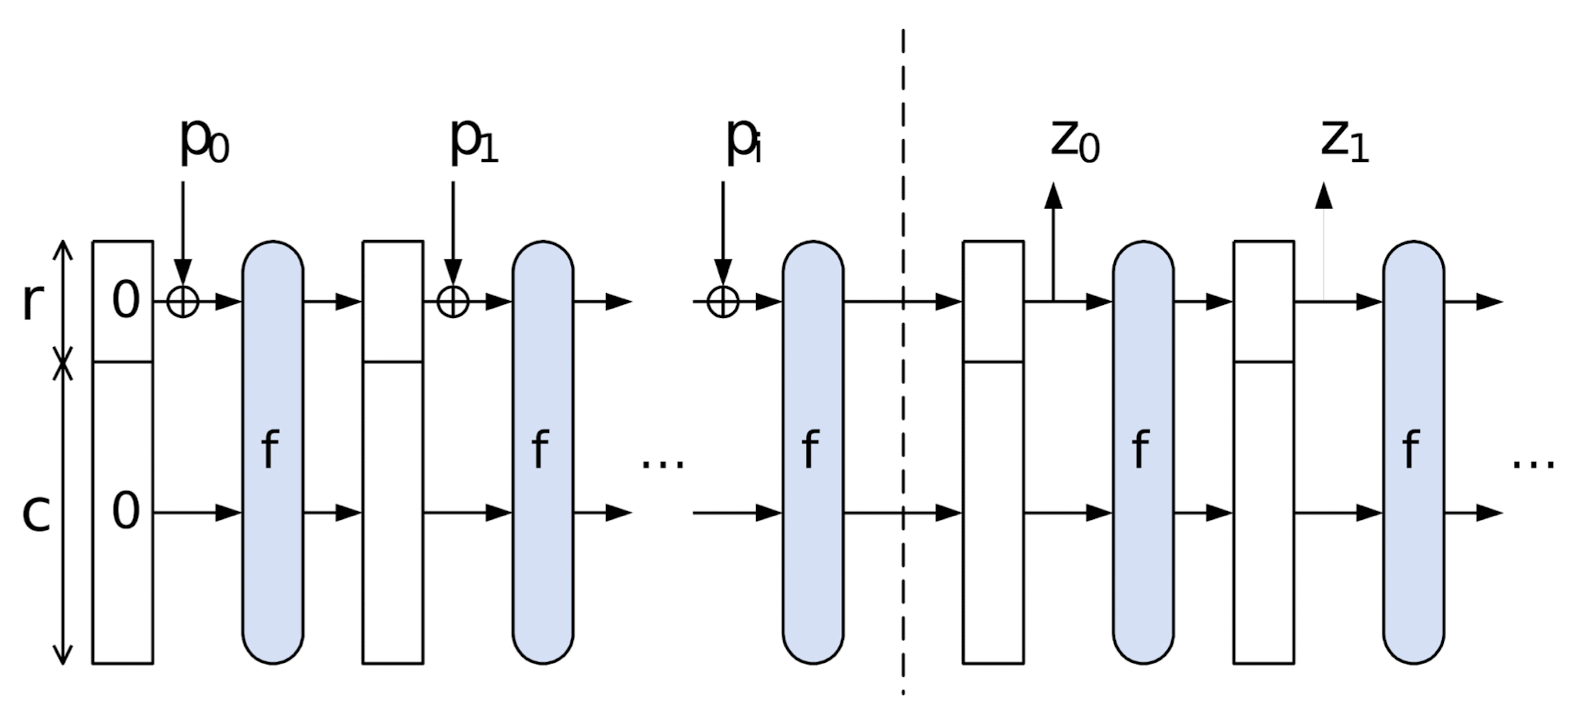
\includegraphics[width=10cm]{figures/f1.png}
\end{figure}
\begin{itemize}
\item $f$ is a permutation (or transformation): no compression
\item $r$ is the bit-rate, $c$ is the capacity
\item Output produced through many "squeezes"
\item Output can have arbitrary length.
\end{itemize}
\newpage
\subsection{Practical constructions}
Generally unkeyed, one function not a family of functions.
\begin{itemize}
\item Practical $\A$ needs to find one collision
\item Much more damaging if some actual collision is found
\item Yet, we can still hope to achieve. "practical security".
\end{itemize}
Security:
\begin{itemize}
\item Collision should cost birthday paradox bound $\frac{q^2}{2*2^n}$
\item $H(x)$ should look random to anyone who did not compute it from $x$.
\end{itemize}
Hash functions in practice are fixed.
\subsection{MD5 [Rivest, 1992]}
\begin{itemize}
\item Produces 128-bit output\\
Birthday paradox: Can be attacked with $2^{64}$ complexity(not good enough for today).
\item Significant weakness found in 2004\\
Today collisions produced in less than a second
\item But still used\\
- Flame cyber-weapon. (2012) authenticated itself as Microsoft validated thanks to MD5 legacy use\\
- Yahoo 1B account breach (2013) showed. MD5 protected passwords.
\end{itemize}
\subsection{SHA-1}
\begin{itemize}
\item Produces 160-bit output
\item Collision found in 2017
\item Phasing out: Browsers stop supporting it in 2017
\end{itemize}

\subsection{SHA-2}
\begin{itemize}
\item A family of successors to SHA-1
\item SHA-256, SHA-384, SHA-512
\item No significant weakness known, most common today.
\end{itemize}

\subsection{SHA-3}
\begin{itemize}
\item NIST standard since 2015 (after 5 years of competition)
\item Slower adoption
\item Sponge construction 
\end{itemize}

\section{MAC construction revisited}
Hash function can help build efficient MAC schemes.\\
Idea: Hash something depending on:
\begin{itemize}
\item The message and a secret
\end{itemize}
e.g., 
\begin{equation*}
t\define \h(k||m)
\end{equation*}

Intuition:
\begin{itemize}
\item Small modifications in message completely change its hash, without knowing the key, nothing can be predicted on tag.
\end{itemize}

\subsection{Building a MAC with a hash function (HMAC)}
\begin{equation*}
	t\define \h((k \xor\, \text{opad})||\h((k \xor\,\text{ipad})||m))
\end{equation*}
Where (opad, ipad) are fixed constants. This construction can be proven secure under some assumptions on the underlying hash function.
\newpage
\subsection{HMAC with \mdt}
\begin{figure}[ht]
    \centering
    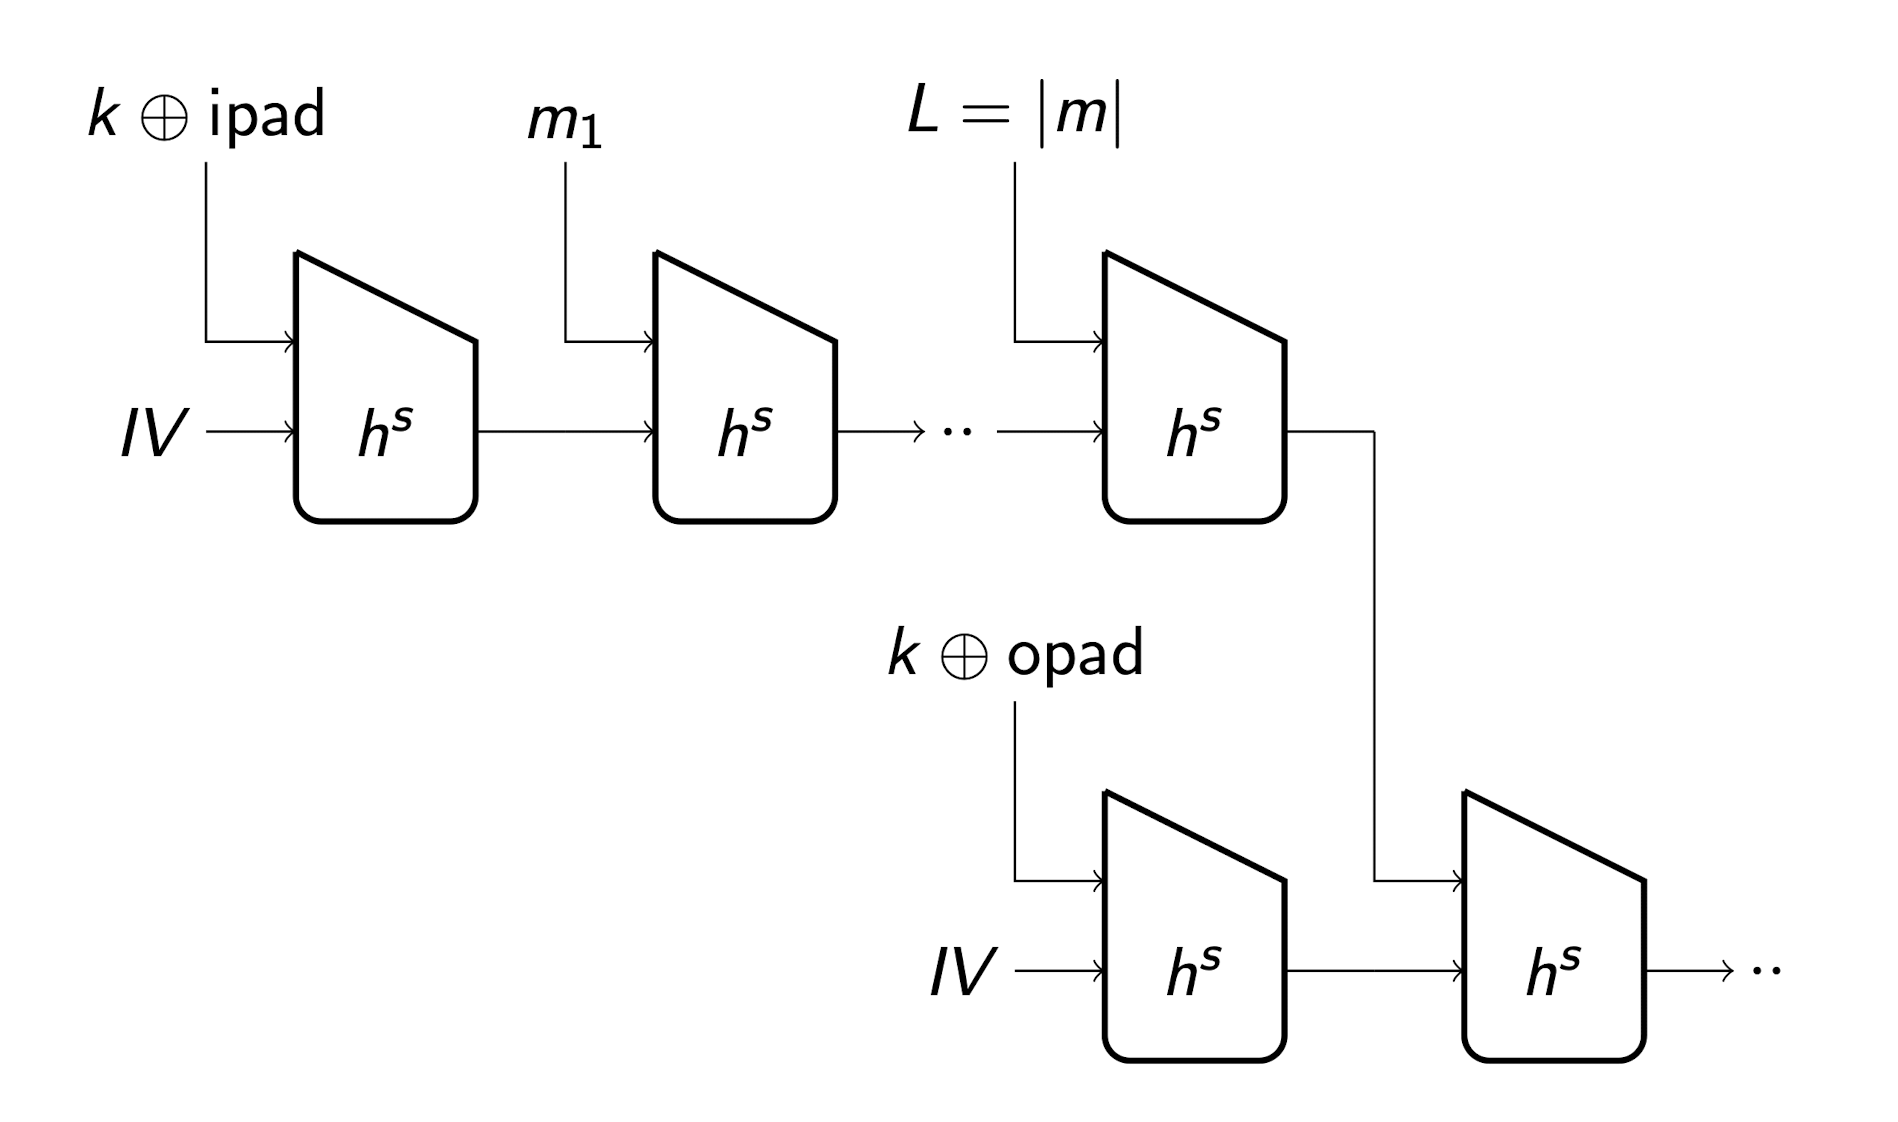
\includegraphics[width=10cm]{figures/f2.png}
\end{figure}

\section{Applications of hash functions}
\begin{itemize}
\item Password storage
\item Create temper-evident logs\\
Maintain a hash chain, any log tempering requires recomputing the whole chain
\item Cryptocurrencies
\item ...
\end{itemize}
\newpage

\section{Practical Constructions of block ciphers}
Why use heuristic schemes?\\
Today, we do not have efficient and provably secure building blocks. If we want to have usable cryptography (that will not consume the main part of the resources), we must use heuristic constructions.

The global approach is that, try to limit the heuristic aspect as much as possible. Use heuristic basic blocks, combined through provably secure constructions.
\begin{itemize}
\item We can limit the uncertainty to a very specific subpart and define exactly what we expect from it.
\item If block gets broken, just replace it by another one, and keep the construction
\end{itemize}

Security for fixed constants $n$ and $l$.

\subsection{Usefulness of PRPs}
Let $F$ be a PRP: $\bset^n \times \bset^n \rightarrow \bset^n$. Then $F$ is also a PRF. \\
Proof idea:
\begin{itemize}
\item PRF attacker queries relayed to and from PRP challenger.
\item Only way to distinguish is that. PRFs have collisions
\item But we can only hope to observe collisions after $2^{n/2}$ queries (birthday paradox)
\end{itemize}
So, it is enough to focus on building good PRPs, and then use them as PRFs as needed.


Let $F$ be a PRP: $\bset^n \times \bset^n \rightarrow \bset^n$. Then $G: s \mapsto F_s(0)||F_s(1)$ is a PRG. 

So, a PRP also gives us a PRG, crazy.

\textbf{Thus, we focus on block ciphers (other name for PRP)}. They are typically defined for just a few values of n (256, 128, ...)

\subsection{Definition of a breaking}
\textbf{Practical requirement is}: Distinguishing from random permutation should be roughly as hard as exhaustive key search.\\
This means, $2^{n/2}$ security would not be enough, even if not PPT. We want to keep the parameters as small as possible.

In the concrete setting we care about the actual complexity of attacks, and not just their asymptotic behavior. Thus, if a cipher with key length $n= 256$ can be broken in time $2^{128}$ the cipher is (generally) considered insecure even though a $2^{128}$ time attack is infeasible.

Furthermore, there is a concern that existence of a better-than-brute-force attack may indicate some more fundamental weakness in the design of the cipher. Brute-force attacks involve trying all possible keys, and if a more efficient attack exists, it suggests a potential flaw.

\subsection{Attacks on a block cipher F}
\begin{itemize}
\item Known plaintext attack: the attacker is given pairs of inputs/outputs $\{(x_i, F_k(x_i))\}$ (for an unknown key k), with the \{$x_i$\} outside the attacker's control.
\item In a chosen-plaintext attack, the attacker is given $\{F_k(x_i)\}$ (unknown key k) for a series of inputs \{$x_i$\} chosen by the attacker.
\item In a chosen-ciphertext attack, the attacker is given $\{F_k(x_i)\}$ for \{$x_i$\} chosen by the attacker, as well as $\{\FI(y_i)\}$ for chosen \{$y_i$\}
\end{itemize}

IMPORTANT:\\
\textbf{A cipher secure against chosen-plaintext attacks corresponds to a pseudorandom permutation, while one secure against chosen-ciphertext attacks corresponds to a strong pseudorandom permutation.}

\section{Substitution-Permutation-Networks (SPNs)}
A secure block cipher (using a random key) must behave like a random permutation. There are $2^l!$ permutations on $l$-bit strings, so representing an arbitrary permutation in this case requires $\log(2^l!) \approx l*2^l$ bits.

Goal: just as evaluating a random permutation at two inputs that differ in only a single bit should yield two (almost) independent outputs (they are not completely independent since they cannot be equal).

This implies that a one-bit change in the input should “affect” every bit of the output. (Note that this does not mean that all the output bits will be changed—that would be different behavior than one would expect for a random permutation. Rather, we just mean informally that each bit of the output is changed with probability roughly half.)
\newpage
\subsection{Gigachad Shannon: The confusion-diffusion paradigm}
Shannon introduced a basic paradigm for constructing concise, random-looking permutations. The basic idea is to construct a random-looking permutation $F$ with a large block length from many smaller random (or random-looking) permutations $\{f_i\}$ with small block length.

Say we want F to have a block length of 128 bits. We can define $F$ as follows: the key $k$ for $F$ will specify 16 permutations $f_1,\dots,f_{16}$ that each have an 8-bit block length. Given an input $x \in \bset^{128}$, we parse it as 16-bytes $x_1\dots x_{16}$ and then set
\begin{equation*}
F_k(x) = f_1(x_1)||\dots||f_{16}(x_{16})
\end{equation*}
These \emph{round functions} $\{f_i\}$ are said to introduce \emph{confusion} into F. It is clear that $F$ defined above is not a pseudorandom. If $x$ and $x'$ differ only in their first bit, then $F_k$ and $F_k(x')$ will differ only in their first byte (regardless of the key).

In contrast, for a truly random permutation changing the first bit of the input
would be expected to affect all bytes of the output.

For this reason, a \emph{diffusion} step is introduced whereby the bits of the output
are permuted, or “mixed,” using a \emph{mixing permutation}. This has the effect of spreading a local change (e.g., a change in the first byte) throughout the entire block. In principle the mixing permutation could depend on the key, but in practice it is carefully designed and fixed.


The confusion/diffusion steps—together called a \emph{round}—are repeated multiple times. This helps ensure that changing a single bit of the input will affect all the bits of the output.

\subsubsection{Example: A two-round block cipher}
First the confusion is introduced by computing the intermediate result $f_1(x_1)||\dots||f_{16}(x_{16})$, where the $\{f_i\}$ depend on the key. 

The bits of the result are then "shuffled", or re-ordered, using a mixing up permutation to give $x'=x_1'\dots x_{16}'$.

Then $f_1'(x_1')||\dots||f_{16}'(x_{16}')$ using possible different $\{f_i'\}$ that again depend on the key, and the bits of the result are again permuted using a mixing permutation to give output $x''$

\subsection{Substitution-permutation networks}
A substitution-permutation network (SPN) can be viewed as a direct implementation of the confusion-diffusion paradigm. 

The difference is that now the permutations ($\{f_i\}, \{f_i'\}$) have a particular form rather than being chosen from the set of all possible permutations. Specifically, rather than having (a portion of) the key $k$ specify an arbitrary permutation $f$, we instead fix a public "substitution function" (i.e., permutation) S called an \emph{S-box}, and then let $k$ define the function $f$ given by $f(x) = S(k \xor x)$. If f takes 8-bit inputs as before, we have thus reduced the number of possibilities for f from $2^8!$ to $2^8$.

\subsubsection{How it works?}
\begin{figure}[ht]
    \centering
    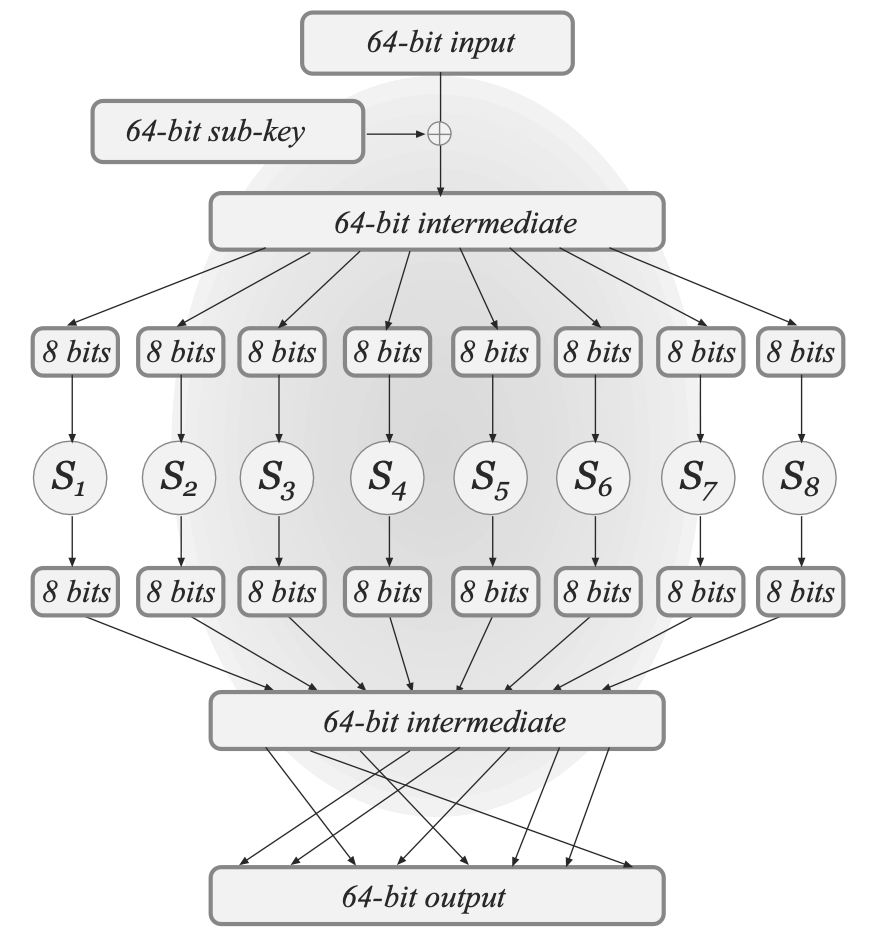
\includegraphics[width=8cm]{figures/f3.png}
\end{figure}

Consider an SPN with a 64-bit block length based on a collection of 8-bit S-boxes $S_1,\dots,S_8$, as above.

Evaluating the cipher proceeds in a series of rounds, where in each round we apply the following sequence of operations to the 64-bit input x of that round (the input to the first round is just the input to the cipher):
\begin{enumerate}
\item \emph{Key mixing:} Set $x\define x\xor k$ where $k$ is the current-round \emph{sub-key}
\item \emph{Substitution:} Set $x\define S_1(x_1)||\dots||S_8(x_8)$, where $x_i$ is the $i$th byte of $x$ 
\item \emph{Permutation:} Permute the bits of $x$ to obtain the output of the round
\end{enumerate}

After the last round there is a final key-mixing step, and the result is the output of the cipher.

Round keys in a block cipher are derived from a master key through a key schedule, where distinct sub-keys are used for each round. The key schedule may be simple, involving subsets of the master key bits, or more complex variations are possible. The master key is also referred to as the actual key of the block cipher.

An r-round SPN has r rounds of key mixing, S-box substitution, and application of a mixing permutation, followed by a final key-mixing step. (This means that an r-round SPN uses r+ 1 sub-keys.)

\emph{Let F be a keyed function defined by an SPN in which the S-boxes are all permutations. Then regardless of the key schedule and the number of rounds, Fk is a permutation for any k.}

\subsubsection{The avalanche effect}
As noted repeatedly, an important property in any block cipher is that a small change in the input must “affect” every bit of the output.

Following two properties hold to induce this effect:
\begin{enumerate}
\item The S-boxes are designed so that changing a single bit of the input to an S-box changes at least two bits in the output of the S-box.
\item The mixing permutations are designed so that the bits output by any given S-box affect the input to multiple S-boxes in the next round.
\end{enumerate}

For a block cipher to be strongly pseudorandom, the avalanche effect should be present in its inverse as well. This means that altering a single output bit should impact every input bit. To achieve this, designing S-boxes to ensure that modifying a single output bit affects at least two input bits is advantageous. Increasing the number of rounds further contributes to achieving the avalanche effect in both directions.
\newpage
\section{AES}
Rijndael
\begin{itemize}
\item 128-bit block cipher
\item SPN (AES-128 has 10 rounds)
\item 3 key sizes: 128, 192, and 256
\end{itemize}


\section{Feistel Networks}
Feistel networks offer another approach for constructing block ciphers. An advantage of Feistel networks over SPNs is that the underlying functions used in a Feistal network (in contrast to S-boxes used in SPNs- need not to be invertible. Sheesh another chad!

This is important because a good block cipher should have "unstructured" behaviour (so it looks random), yet requiring all the components of a construction to be invertible inherently introduces structure. Requiring invertibility also introduces an additional constraint on S-boxes, making them harder to design.

A Feistel network operates in a series of rounds. In each round, a keyed round function is applied. Round functions need not be invertible. They will typically be constructed from components like S-boxes and mixing permutations, but a Feistel network can deal with any round functions irrespective of their design.
\begin{figure}[ht]
    \centering
    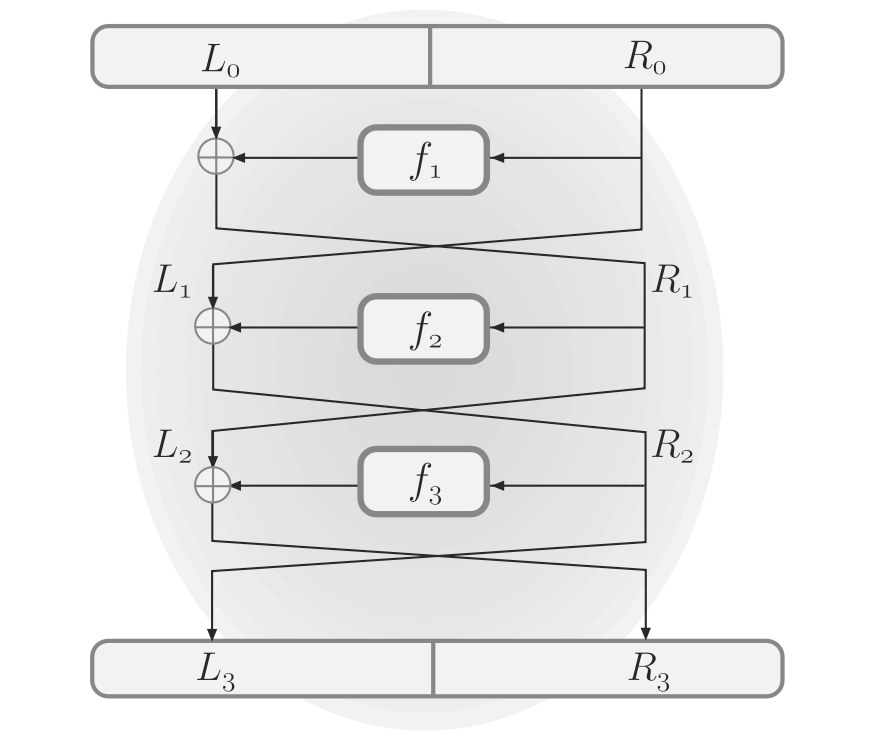
\includegraphics[width=8cm]{figures/f4.png}
    \caption{A three round Feistal network }
\end{figure}

In a (balanced) Feistal network with $l$-bit block length, the $i$th round function $\hat{f}_i$ takes as input a sub-key $k_i$ and an $l/2$-bit string and generates an $l/2$-bit output. As in the case of SPNs, a master key $k$ is used to derive the sub-keys for each round.

When a master key is chosen, thus determining each sub-key $k_i$. We define:
\begin{equation*}
f_i: \bset^{l/2} \rightarrow \bset^{l/2} \text{ via } f_i(R) \define \hat{f}_i(k_i,R)
\end{equation*}

Note that the round functions $\hat{f}_i$ are fixes and publicly known, but the $f_i$ depend on the master key and so are not known to the attacker.

The $i$th round operates as follows:
\begin{itemize}
\item The $l$-bit input to the round is divided into two halves $L_{i-1}$ and $R_{i-1}$ (Left and Right halves)
\item The output of the round  $L_{i},R_{i}$ is
\begin{equation*}
L_i \define R_{i-1} \text{ and } R_i \define L_{i-1} \xor f_i(R_{i-1})
\end{equation*}
\end{itemize}
In an r-round Feistel network, the $l$-bit input to the network is parsed as (L0,R0), and the output is the $l$-bit value $(L_r,R_r)$ obtained after applying all r rounds. As in the figure above.

\subsection{How to invert this beast?}
A Feistal network is invertible regardless of the $\{f_i\}$. To show this we only need to show that each round of the network can be inverted if $\{f_i\}$ are known. Given output $(L_i,R_i)$ of the $i$th round, we can compute $(L_{i-1},R_{i-1})$ as follows:
\begin{itemize}
\item Set $R_{i-1}\define L_i$
\item Then
\begin{equation*}
L_{i-1} \define R_i \xor f_i(R_{i-1})
\end{equation*}
Damn, it actually works. Crazy.

It can be proven that: If $f_i$ is a PRF:
\begin{itemize}
\item Then a 3-round Feistel network is a PRP
\item And a 4-round Feistel network is a strong PRP.
\end{itemize}

Advantages:
\begin{itemize}
\item More flexibility in the choice of $f_i$
\item Same hardware/software can be used for encryption and decryption.
\end{itemize}

Examples: DES, Camellia, ...

\section{DES}
\begin{itemize}
\item US encryption standard 1977 from IBM / NSA
\item Feistal network
\item 64-bit block cipher
\item 56-bit keys
\end{itemize}
Not secure anymore. Sizes are too short for today's computing power.


\end{itemize}






























\end{document}